\documentclass[./../SoftwareEngineering.tex]{subfiles}

\begin{document}
	\section{Thiết kế trong lĩnh vực lập trình}
	Thiết kế phần mềm là một phần quan trọng của kỹ nghệ phần mềm và được áp dụng đối với tất cả các mô hình phát triển phần mềm. Các yêu cầu phần mềm ban đầu sẽ được phân tích và tiến hành mô hình hóa, thì thiết kế phần mềm chính là bước cuối cùng trong hoạt động mô hình hóa chuẩn bị cho giai đoạn xây dựng ( sinh mã nguồn và thử nghiệm).
	\begin{figure}
		\centering
		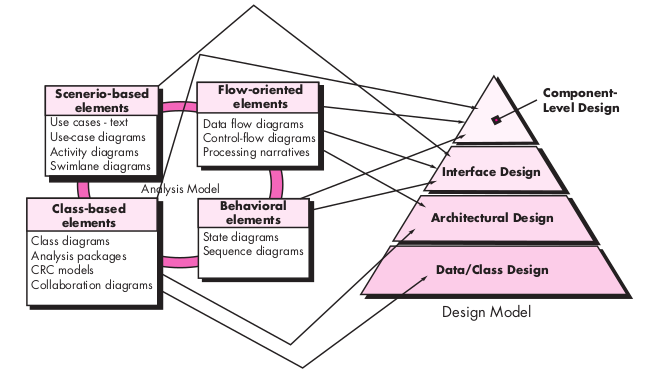
\includegraphics[width=\textwidth]{figure_8_1.png}
		\caption{Chuyển mô hình yêu cầu thành mô hình thiết kế}
		\label{fig8_1}
	\end{figure}
	
	Mỗi một thành phần của mô hình yêu cầu (Chương 6 và 7) sẽ cung cấp thông tin cần thiết để tạo ra bốn mô hình thiết kế quy định cho một đặc tả thiết kế hoàn chỉnh. Luồng thông tin trong quá trình thiết kế phần mềm được minh họa trong Hình 8.1. Mô hình yêu cầu, được thể hiện qua các thành phần dựa trên kịch bản (scenario-based), dựa trên lớp(class-based), hướng luồng (flow-oriented) và hành vi (behavioral), cung cấp cho công việc thiết kế. Sử dụng ký hiệu thiết kế và phương pháp thiết kế sẽ được thảo luận trong các chương sau, thiết kế được chia thành các nội dung:  thiết kế cấu trúc dữ liệu (data/class), thiết kế kiến trúc (architectural), thiết kế giao diện (interface) và thiết kế thành phần (component).
	
	Thiết kế cấu trúc dữ liệu: biến đổi các mô hình lớp (Chương 6) thành hiện thực hóa lớp thiết kế và các cấu trúc dữ liệu cần thiết để thực thi phần mềm. Các đối tượng, các mối quan hệ được xác định trong sơ đồ CRC cũng như những nội dung chi tiết được mô tả bởi các thuộc tính lớp cùng với các ký hiệu khác đều cung cấp cơ sở cho việc thiết kế dữ liệu. Một phần của thiết kế lớp có thể xảy ra kết hợp với thiết kế kiến trúc phần mềm. Thiết kế lớp có thể đi vào chi tiết hơn khi mỗi thành phần của phần mềm được thiết kế.
	
	Thiết kế kiến trúc: xác định mối quan hệ giữa cấu trúc chính của phần mềm,kiểu kiến trúc(architectural styles) và mẫu thiết kế (design patterns) cái mà được xem là một mô tả hay một sườn (template) mô tả phong cách thiết kế [Sha96]. Đại diện cho một thiết kế kiến trúc framework của hệ thống computer-based- là một thiết kế có nguồn gốc từ mô hình yêu cầu.
\end{document}